\section{Introduction}
\label{sec:introduction}

\begin{wrapfigure}{r}{0.5\textwidth}
\vspace{-6mm}
\begin{center}
    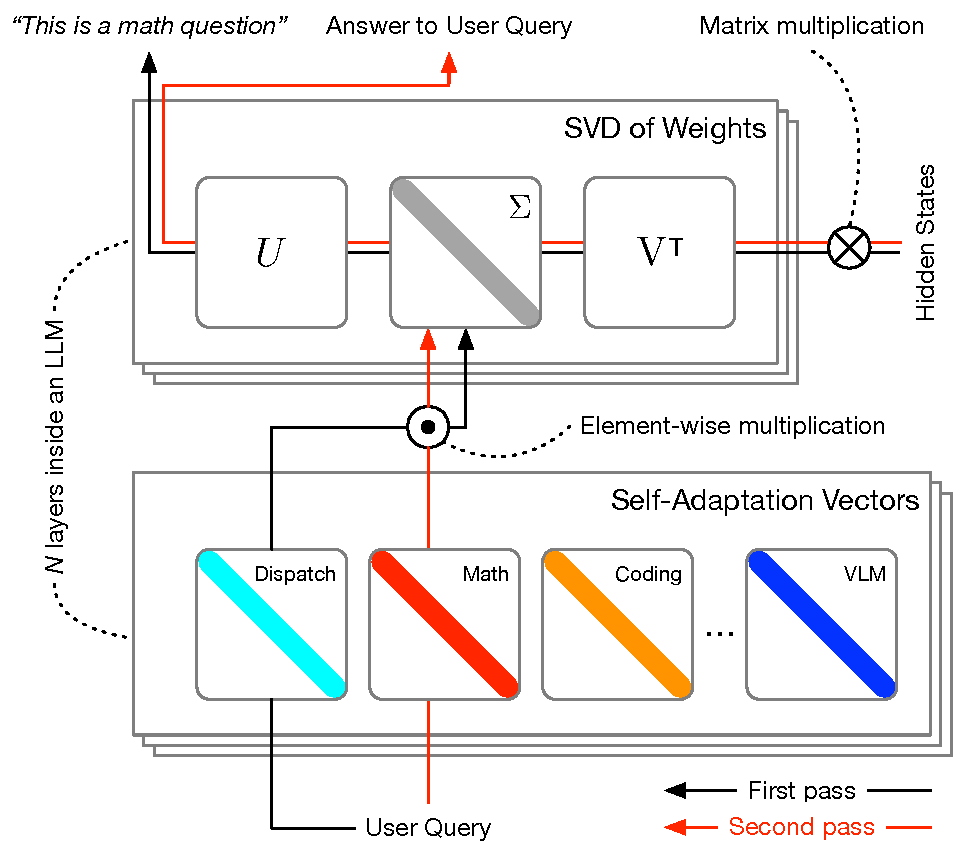
\includegraphics[width=0.5\textwidth]{images/cover.pdf}
  \end{center}
  \vspace{-4mm}
  \caption{\textbf{Overview of \implname.} In training, we tune the singular values of the weight matrices to generate a set of ``expert'' vectors specializing in different tasks. In inference, a two-pass process is adopted where the first applies the expert and the second generates the answer.}
  \label{fig:cover}
  \vspace{-4mm}
\end{wrapfigure}

Self-adaptive large language models (LLMs) would represent a significant advancement in artificial intelligence, enabling real-time adaptation to various tasks and contexts.
While compositionality and scalability are crucial for effective adaptation, current LLM training methodologies fall short of achieving both these properties simultaneously.
Our research aims to present a solution to address these gaps.

In principle, the first step toward achieving self-adaptive LLMs can be realized through the development of specialized expert modules, each fine-tuned~\citep{kaplan2020scaling} via techniques such as low-rank adaptation (LoRA)~\citep{hu2021lora}. 
However, several challenges need to be addressed to make this approach both scalable and compositional: (1) multiple expert modules significantly increase the number of parameters; (2) expert modules are often prone to overfitting; and (3) flexible composition of these experts is still an open problem.

To overcome these limitations, we first propose \svdacro, a novel parameter-efficient fine-tuning (PEFT) method to obtain effective building blocks for self-adaptation.
\svdacro works by extracting and selectively tuning only the singular values within the model's weight matrices.
By focusing on this essential and principled parameterization, our approach mitigates the risk of overfitting, drastically reduces computational demands, and allows for inherent compositionality.

We then introduce our full \implname framework, which entails a two-pass inference mechanism to produce dynamically adapted weights targeted for the test-time conditions (Figure~\ref{fig:cover}).
We design three different adaptation strategies that can be used within \implname, which we show provide monotonic performance benefits with increasing access to the test-time conditions.
We evaluate \svdacro and the full \implname framework through extensive experiments across a diverse range of LLMs and tasks.
\svdacro outperforms traditional efficient fine-tuning methods like LoRA on domain-specific datasets with far fewer parameters. 
\implname further improves performance, even for out-of-distribution tasks like visual QA. 
Our analysis even shows that \implname allows the reuse of \svdacro experts across different LLMs. In summary, our key technical contributions are: 
\vspace{-2mm}
\begin{itemize}
\item The development of \implname as a pivotal self-adaptation framework for LLMs, providing a blueprint to adapt the behavior of LLMs from a growing set of pre-trained skills.
\item The introduction of \svdacro, a novel PEFT method trainable with RL on small datasets, producing compact expert vectors with inherent compositionality.
\item The implementation of three adaptation strategies, effectively dispatching \svdacro-trained experts with properties designed to cope with different deployment scenarios.
\end{itemize}

\vspace{-2mm}